\documentclass[12pt,a4paper]{report}

\documentclass{article}
\usepackage{listings,xcolor}
\usepackage{inconsolata}
\usepackage{lmodern}  % for bold teletype font
\usepackage{amsmath}  % for \hookrightarrow

\definecolor{dkgreen}{rgb}{0,.6,0}
\definecolor{dkblue}{rgb}{0,0,.6}
\definecolor{dkyellow}{cmyk}{0,0,.8,.3}

\lstset{
  language        = php,
basicstyle      = \small\ttfamily,
keywordstyle    = \color{dkblue},
stringstyle     = \color{red},
identifierstyle = \color{dkgreen},
commentstyle    = \color{gray},
emph            =[1]{php},
emphstyle       =[1]\color{black},
emph            =[2]{if,and,or,else},
emphstyle       =[2]\color{dkyellow}
breaklines=true,
postbreak=\mbox{\textcolor{red}{$\hookrightarrow$}\space},
}

\setlength{\topmargin}{-2cm}
\setlength{\oddsidemargin}{0cm}
\setlength{\textheight}{24cm}
\setlength{\textwidth}{16cm}
\usepackage{graphicx}
\usepackage{float}
\renewcommand{\baselinestretch}{1.35}
\setlength{\parindent}{2cm}
\setlength{\parskip}{.1cm}
%\usepackage{mathptmx}
\usepackage{tabto}
\usepackage[utf8]{inputenc}
\usepackage{listings}
% for url entries

\usepackage{xurl}
\usepackage{enumitem}
\usepackage{sectsty}
\DeclareUnicodeCharacter{2212}{~}
\begin{document}
% following is the title page
\begin{titlepage}
\begin{center}
\begin{large}
			\textbf{\large  MY TOWN HOME SERVICES}\\[.75cm]
		\end{large}
		\textbf{ \large A}\\[.45cm]
		\textbf{ \large Major Project Report}\\[.45cm]		
		\textit{\large Submitted in fulfillment of\\ the requirements for the award of the degree of}\\[.6cm]
\textbf{\large  {Bachelor of Technology\\[.1cm] in}}\\[.1cm]
\textbf{\large {Computer Science and Engineering }}\\[.25cm]
\textup{\large Submitted by}\\[.25cm]
 \begin{table}[ht]
			\begin{center}
			       \begin{tabular}{l r}
				{\small \textbf{KANDUKOORI VIKRAM}} & {\small \textbf{(18SS5A0509)}}\\
				{\small \textbf{BURRA MADAN}} & {\small \textbf{(18SS5A0502)}}\\
				{\small \textbf{RAVALI DHONI}} & {\small \textbf{(18SS5A0504)}}\\
				{\small \textbf{BHUKYA MANISHA}} & {\small \textbf{(17SS1A0506)}}\\
			\end{tabular} 
			\end{center}{}
			
		\end{table}

\vspace{0.45cm}
\textup{{\large Under the guidance of}}\\
\textbf{{\large  Mr.P. KRUPA SAGAR}}\\
%\textup{Head of Department}\\
\begin{center}

			
\includegraphics[scale=0.6]{logoj}
		\end{center}
%\vspace{0.5cm}
\textup {\large{Department of Computer Science and Engineering}}\\
\normalsize
%\vspace{0.5cm}
\textup {{JNTUH College of Engineering,Sultanpur}}\\
\vspace{0.04cm}
\textup{\footnotesize {Sultanpur(V),Pulkal(M),Sangareddy district,Telangana-502273 }}\\[.23cm]
\textup{\small{June 2021}}
\end{center}
\end{titlepage}
\pagenumbering{roman}
	\addcontentsline{toc}{chapter}{Certificate}
	
\newpage
\begin{titlepage}
\begin{center}
\begin{large}
            \textsc{\large JNTUH COLLEGE OF ENGINEERING SULTANPUR}
            \textit{\large Sultanpur(V),Pulkal(M),Sangareddy-502273,Telangana.}\\[0.25]
            
\end{large}
\begin{center}
    
\includegraphics[scale=0.6]{logoj}
    \end{center}
    \textit{\large Department of Computer Science and Engineering}\\ 
    \vspace{1cm}
\textit{\large\boldsymbol{Certificate}}\\[1.25]    
\end{center}
\vspace{0.5cm}
{\large This is to certify that the Major Project work entitled \textbf{"MY TOWN HOME SERVICES"} is a bonafide work carried out by the team consisting of  \textbf{KANDUKOORI VIKRAM} bearing Roll no.\textbf{18SS5A0509}, \textbf{BURRA MADAN} bearing Roll no.\textbf{18SS5A0502}, \textbf{RAVALI DHONI} bearing Roll no.\textbf{18SS5A0504}, \textbf{BHUKYA MANISHA} bearing Roll no. \textbf{17SS1A0506} in partial fullfillment of the requirements of  the degree of \textup{BACHELOR OF TECHNOLOGY} in \textup{COMPUTER SCIENCE AND ENGINEERING} discipline to Jawarlal Nehru Technological University,Hyderabad during the academic year 2020-2021.\\
The results emboided in this report have not been submitted to any other University or Institute for the award of any degree or diploma.}\\

\vspace{0.5in}
% Bottom of the page
\noindent
\textbf{Project Guide}\hspace{3.0in}\textbf{Head of The Department}\\
\hspace{2.5in}
\textbf{Mr.P. KRUPA SAGAR}\hspace{2.3in}\textbf{SHRI JOSHI SHRIPAD}\\
\hspace{0.3in}\textbf{Assistant Professor(C)}\hspace{2.7in}\textbf{Associate Professor}\\
\vspace{0.3in}
\begin{center}
    \textbf{PRINCIPAL}\\
\end{center}

\newpage
\pagenumbering{roman}
	\setcounter{page}{2}
\addcontentsline{toc}{chapter}{Declaration}

\begin{center}
	%\vspace*{.25 cm}
	\textbf{\textit{\Large Declaration}}
\end{center}
	\vspace{.5 cm}
	\large
	We declare that the Major Project report work entitled \textbf{”MY TOWN HOME SERVICES”} submitted by us in the Department of Computer Science and Engineering,JNTUH College of Engineering Sultanpur in partial fulfillment of the degree for the award of Bachelor of Technology,Computer Science and Engineering is a bonafide work,carried out by us under the supervision of Mr.P. Krupa sagar,Assistant Professor(C). Also,We declare that the matter embodied in this report has not been submitted by us in full or partial there of for the award of any degree or diploma of any other University or Institution previously.\\\\

 \begin{table}[ht]
			\begin{flushright}
			       \begin{tabular}{l r}
				{\large \textbf{KANDUKOORI VIKRAM}} & {\large \textbf{(18SS5A0509)}}\\
				{\large \textbf{BURRA MADAN}} & {\large \textbf{(18SS5A0502}})\\
				{\large \textbf{RAVALI DHONI}} & {\large \textbf{(18SS5A0504)}}\\
				{\large \textbf{BHUKYA MANISHA}} & {\large \textbf{(17SS1A0506)}}\\
			\end{tabular} 
			\end{flushright}{}
			
		\end{table}

\newpage
\addcontentsline{toc}{chapter}{Acknowledgement}

\begin{center}
		%\vspace*{.5 cm}
	\textbf{\textit{\Large Acknowledgement }}
\end{center}
	%\vspace{.5 cm}
	\large
		%\vspace{0.5cm}
We wish to take this opportunity to express our deep gratitude to all those who helped us in various ways during our major project report work.It is our pleasure to acknowledge the help of all those individuals who where responsible for foreseeing the successful completion of this major project.We wish to express our gratitude to all those who helped to complete our major project report.\\
We express our sincere gratitude to \textbf{Prof. B. BALU NAIK},Principal of JNTUHCES for his support during the course period.\\
We sincerely thank \textbf{Prof. V. VENKATESWARA REDDY},Vice Principal of JNTUHCES for his kind help and co-operation.}\\
We are thankful to \textbf{SHRI JOSHI SHRIPAD},Associate Professor and Head of the Department of Computer Science and Engineering of JNTUHCES for his effective suggestions during the course period.\\
We would like to convey our profound thanks to our \textbf{Dr.B.V. RAM NARESH YADAV},Associate Professor of Computer Science Department  and his challenges bought this work towards completion.\\
Our special thanks to our Guide \textbf{Mr.P. KRUPA SAGAR},Assistant Professor(C) for his suggestions and good understanding in the completion of this project work.\\
Finally, special thanks to our parents for their support and encouragement throughout this course.
\vspace{0.5cm}
 \begin{table}[ht]
			\begin{flushright}
			       \begin{tabular}{l r}
				{\large \textbf{KANDUKOORI VIKRAM}} & {\large \textbf{(18SS5A0509)}}\\
				{\large \textbf{BURRA MADAN}} & {\large \textbf{(18SS5A0502}})\\
				{\large \textbf{RAVALI DHONI}} & {\large \textbf{(18SS5A0504)}}\\
				{\large \textbf{BHUKYA MANISHA}} & {\large \textbf{(17SS1A0506)}}\\
			\end{tabular} 
			\end{flushright}{}
			
		\end{table}

\newpage
\addcontentsline{toc}{chapter}{Abstract}
\begin{center}

\textbf{\textit{\Large Abstract}}\\[1cm]
\end{center}
{\large The generic scenario that has always been the case when it comes to household services, namely plumbing, electrical, carpentering, house cleaning and gardening is that, one sets up a call to the service provider and resolve these domestic issues. Our project here aims at targeting the town spaces for the implementation. Urban spaces are pretty much the first priority usually for anyone to practicalize any idea, we wanted to make a bottom up approach by specifically taking the town areas. To familiarise with the project, it develops a website that would contain all the required elements to cater to the needs of the customer which needs to be resolved. A website like this would make a platform for employment opportunities and progress the lives of service providers along with the speedy and handy resolution for the costumers. This website particularly has features of the location, time of appointment, details of contact, effective tackling of online security related issues, navigation and advertisements.

\newpage
\addcontentsline{toc}{chapter}{List of Figures}
\listoffigures

\newpage
\renewcommand{\baselinestretch}{0.5}
\tableofcontents
	\addtocontents{toc}{}
	\clearpage
	
\newpage
\renewcommand{\baselinestretch}{1.25}
\pagenumbering{arabic}
\chapter{INTRODUCTION}
\Large

\section{ General Description }
\vspace{0.5cm}
Our platform, inspired by the ever-significant reference in the Indian household context, is
the one-stop solution for all your daily needs. Be it the most minuscule of the most daunting
Household Service, we serve you with the best quality, highly reliable, and recommended
Independent Professionals and Enterprise service providers.
In the present scenario, people are buried up in heavy work culture, as everyone is engaged with
busy schedules and hectic tasks which make them deviate from family life. If any issues encounter
unexpectedly, it distracts them and makes them choose over the work they have to accomplish
primarily.\\ 
It is important to manage both professional and family life. In such circumstances, every one of us
would have fantasized about a kind of house which doesn’t have any leaks in pipes, if it doesn’t have
any mess in fixing furniture and a kind of house which never face any maintenance issues and every
one of us has thought that life would be much better if no point of issue arises in getting service at
your doorstep and if there is no mess in bargaining labor for home service. In such situations,
E-Commerce plays a vital role in today’s life as it has so many advantages in our life because it
makes it convenient in the daily life of the people.\\ 
So, giving a thought to that aspect of life is to design and develop a system that provides many
services at your doorstep in just one click. A system that provides a variety of services like
plumbing, house cleaning,electric, carpentering and gardening. To make it comfortable for all the
users our system also provides an environment that offers ease in accessing our services. A very
simple process is carried out to book a service. The system is versatile as service can be booked
from everywhere to anywhere you desire.\\
\section{ Objectives and Scope of the Project }
\vspace{0.5cm}
\subsection{Objectives}
\vspace{0.5cm}
\begin{itemize}
	\item Collecting data of various plumbers,carpenters,electricians,house cleaning persons,gardeners like their experience, available time, their domain.
	\item Providing desired plumbers,carpenters,electricians,house cleaning persons and gardeners.
	\item Innovative platform to book required service in required domain.
	\item Build a user friendly website to book a required service.
	\item Easy and efficient search by name or domain of the service provider.
	\item Saving time for customers in booking service provider.
\end{itemize}
\vspace{0.5cm}
\subsection{Scope}
\vspace{0.5cm}
The scope of our project is to designing a complete environment to provide a safe and user friendly environment for online service booking. The main aim of the project is to provide an easy to use application for services provided for customer.\\
We often get frustrated while taking the appointment of service provider because there the many problems will occur,  like the service provider is busy at somewhere else or  he is not receiving our call. So in this project we will remove this headache.\\
\newpage
\section{ Project Definition }
\vspace{0.5cm}
In this fast growing technology, we still have to take the appointment of person who solve the problems related to our daily life like plumbing,carpentering, electrical,house cleaning and gardening etc.
\\
To take the appointment of service provider we have to call him or with the personal meeting we can meet him, and it is not sure that we get the appointment of the service provider at a time because there are many problems occur, like the service provider is busy at somewhere else or he is not present at his office when we go there or he wants heavy cost for fix the problem etc.\\
We are not getting any service on time and also not proper changes of services. It is also not secure in terms of safety concern.\\
To overcome these type of problem we are going to make our website where the people get appropriate result.\\
This website is very dynamic and very easy to understand. The interface of the website is very easy and anybody can easily work on it. This website can provide all the description and important information about the problem.\\
The household service website is also very useful because the customer don’t have to visit to service provider’s office, he/she can easily book his/her order via this website and he/she can also pay the payment online in this website. So he/she can book order without any kind of disturbance. Our website is secured with QR code. It will provide security for the customer.
To make this website work successfully we have used html,css,bootstrap,php,and My sql as the database management environment.
\vspace{0.5cm}
\section{ Organization and Project Report  }
\vspace{0.5cm}
Generally, the project organization is the structuring, organization and configuration as well as project process according to the plan. It provides the teamwork of the participants proceed as efficient as possible according to the inserted rules, standards and values of the project. The roles and responsibilities are divided, the rules of the team work are determined and the information system is defined during the project organization.\\ \\ The project organization is divided into three areas of competence and responsibility. The project leadership is responsible for the whole management of the project and the project team implements the actual project. The third area is a project board, which is a supreme decision-making body, can define the project successes or cancel a project.
\newpage
\chapter{ LITERATURE SURVEY}
We have observed so many problems which are occur in our daily routine, for example the problem of electricity, if the electricity goes there are many problems occurs in our work, like we cannot charge the phones, batteries etc. The electric devices which are used in kitchen cannot be work.In existing system the whole process is offline and customer can not get proper solution for the problem. The existing system is not available for 24 hours, so the customer can not get solution for any time.We also observe the problem of plumbing at our home. In that situation what we will do. Firstly we call the Plumber and take his appointment if available or we directly meet him for the appointment to fix the problem. This process is very time consuming and it is not sure that we get the appropriate solution for our problem.\\ \\
By observing these type of problems we thought that, how can we get the solution of these type of  problem in easy and appropriate way, then we get an idea to developing our website where people can get any type of services like plumbing, electrical, house cleaning, carpentering, gardening.In this stage of technology our website is very simple and easy to understand. 
\vspace{0.5cm}
\section{ Existing Approaches/System }
\vspace{0.5cm}
There are quite a good number of website available these days which aims at providing home services but these services seem to be highly inefficient in reaching out to last number of customers or in solving the issues of the existing customers.\\
\section{ Drawbacks in Existing System }
\vspace{0.5cm}
\begin{itemize}
	\item Approximately 40\% of the service providers quote unreasonable pricing.
    \item Approximately 30\% of the service providers are amateurs, and not Professionally trained
    \item Approximately 20\% of the service providers are affordable and professionally trained but are always
    engaged with other commitments
    \item Only 10\% of the service providers are affordable, professionally trained, and available to engage in
    work immediately. Our Business Model precisely focuses on this section and ensures that you are served only from the best.
\end{itemize}
\section{ Motivation for Proposed System }
\vspace{0.5cm}
The service providers are affordable, professionally trained, and available to engage in work immediately. Our Business Model precisely focuses on this section and ensures that you are served only from the best.\\
\begin{itemize}
	\item House hold services are easily available.
	\item To provide house hold services any time.
	\item Saving of time.
	\item Make available house hold services through website
	\item It shows the experience and their details with their available time.
	\item  This is web based, so it is easy to access after deployment.
\end{itemize}
\newpage
\chapter{ REQUIREMENT SPECIFICATIONS }

\section{ Overall Description of the Project Product Perspective}
\vspace{0.5cm}
The Web based concepts have great real-time applications in various
fields.The aim of project is to provide the services to the customers at reasonable rate. This project provide the facilities to the customer such as registration, display profile of service provider, advertisement, QR code, map navigation etc.
\begin{enumerate}
	\item Input: Login of user and search of home services by same or required domain.
	\item Php and Javascript code: Input values will be given to this and the list of home services available on that date will be given to the output.
	\item Output: User can select any home service and book at anytime from anywhere.
	\vspace{0.5cm}
\end{enumerate}
\raggedright
\textbf{Product Functions}\\
\vspace{0.5cm}
It has two different logins which are customer and service provider, both has authorized account in this platform. The customers has to search for the required service provider in this platform after their registration and login. Then it shows the list of all service providers who are available otherwise it shows no matches found. After this we are just use clock stay to book any service provider in that list. The service provider gets the Mail notification about it, and our details get sends to him.
\section{ Functional \& Non-functional Requirements }
\vspace{0.5cm}
\subsection{ Specifications}\\
\vspace{0.5cm}
Every project comes with its own set of requirements. Those requirements need to be accomplished in order to bring the project to life with all the modules running smoothly. This section of requirement specifications discusses the software requirements of project My Town Home Services.\\
\newpage
\textbf{Functional Requirements}
\vspace{0.5cm}
\begin{enumerate}
	\item Customers have to give data for login and searching.
	\item The system shall allow the customer to upload data.
	\item The system shall show list after searching.
	\item The system shall provide the correct output i.e. The list of all  service providers who are available.
	\vspace{0.5cm}
\end{enumerate}
\textbf{Non-Functional Requirements}\\
\vspace{0.5cm}
\begin{enumerate}
	\item Scalability: System should be able to handle large number of users. The system is capable enough to work properly.
	\item Speed: The application should be fast. It should not slow down with the increase of number of users.The system should be quick enough to be able to respond to user actions with a short period of time.
	\item Usability: User interface should be simple and clear to break understand to end user. Not every step of this project user seems to be familiar with the interfaces as they are easy to use.
	\item Availability: The system should be available at every moment to the user. It should be ensured that their should be minimum or no downtime to ensure better user experience for customers.
	\item Reliability: The system should be reliable and shows correct requests if a user performs any actions.
	\item Testability: The application is tested for validation, uploading images, message structures and works fine.
\end{enumerate}
\newpage
\section{ Design Specification }
\vspace{0.5cm}
\subsection{Class Diagram}
The class diagram is the main building block of object-oriented modeling. It is used for general conceptual modeling of the structure of the application, and for detailed modeling, translating the models into programming code. Class diagrams are the only diagrams which can be directly mapped with object-oriented languages and thus widely used at the time of construction.\\
\vspace{1.0cm}
\begin{figure}[h!]
	\begin{center}
		 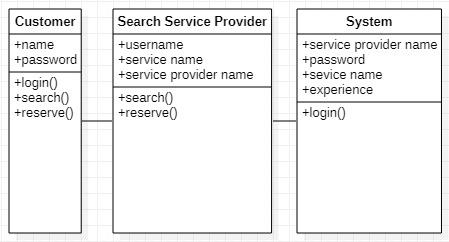
\includegraphics[width=\linewidth]{clas.jpeg}
	\end{center}
	\caption{Class Diagram for My Town Home Services}
\end{figure}
\subsection{ Sequence Diagram with Timelines}
\vspace{0.5cm}
Sequence diagram of this project consist of customer,service provider and a system(PHP server) as participant. The sequence of actions that are performed by the application is showed in detail in the diagram below.\\ 
\vspace{1.0cm}
\begin{figure}[h!]
	\begin{center}
		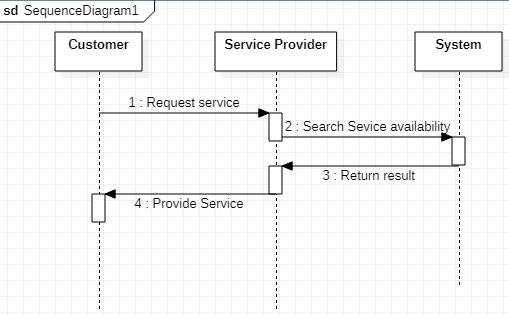
\includegraphics[width=\linewidth]{se.jpeg}
	\end{center}
	\caption{Sequence Diagram for My Town Home Services}
\end{figure}
\newpage
\subsection{ Methodology (With Flowchart) }
\vspace{0.5cm}
It has two different logins which are customer and service provider. The customer i,e user enters his login credentials. If those credentials matches with the his/her original details in the database then he/she allowed to login.\\ \\
\vspace{0.20cm}
After login the user searches for his required service provider in the search bar. If he wants a particular service provider which he knows him before he can search that service provider by his name and can reserve him in the list. If he doesn't know anything about service providers and only wants the service provider in his own choice of domains then he searches via domain. Then a list of service providers who are working under that domain will be displayed according to the data collected from service providers when they were registered. If there are no records matching the user needs then it shows no matches found. The user can select a particular service provider through that list based on his skills, work, experience and available time. If the user wants him, he can reserve him.\\ \\ After reserving the service provider a notification which had the details about this will be send to that service provider via Mail, so that he get to know about it and can contact the user after it for the service. This is the total process involved in this method and it is very easy and efficient way to handle all things.\\
\vspace{0.20cm}
The steps involved in this process are depicted below as a Flowchart. It has clear information of steps to follow.\\
\begin{figure}[h!]
	\begin{center}
		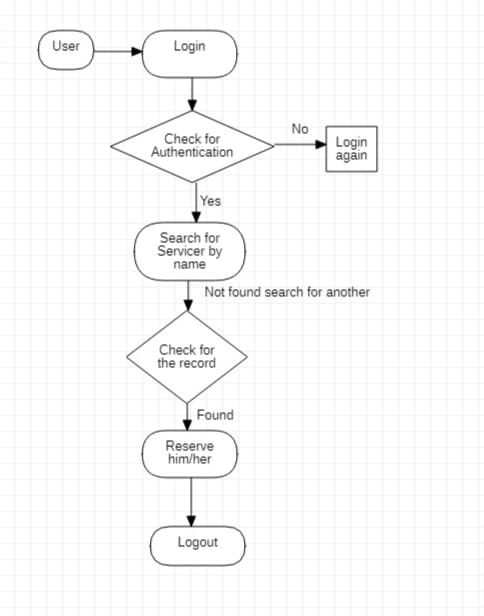
\includegraphics[width=\linewidth]{flow.jpeg}
	\end{center}
	\caption{Activity Diagram for My Town Home Services}
\end{figure}
\newpage
\section{ Software and Hardware Requirements }
\vspace{0.5cm}
The hardware and software component of a computer system that are required to install and use software efficiently. The software manufacturer will list the system requirements on the software package. If your computer system does not meet the system requirements then the software may not work correctly after
installation.\\
System requirements for operating systems will be hardware components, while  other application software will  list both hardware and operating  system requirements. System requirements are most commonly seen listed as minimum and recommended requirements. thee minimum system requirements need to be met for the software to run at all on your system, and the recommended system requirements,if set, will offer better software usability.\\ \\
\vspace{0.75cm}
\textbf{Software Requirements}
\vspace{0.5cm}
\begin{itemize}
	\item Operating System: Windows 2000 or higher versions
	\item Web Browser
	\item Apache Server
	\item Xampp server
	\item Database : Mysql\\
\end{itemize}
\newpage
\textbf{Hardware Requirements}
\vspace{0.5cm}
\begin{itemize}
	\item Processor: Standard processor with a speed of 1.8 GHz
	\item RAM: Minimum of 512 MB RAM
	\item Hard Disk: Minimum 80 GB
	\item Monitor: Standard colour monitor
\end{itemize}
\newpage
\chapter{ IMPLEMENTATION }
\section{Modules Description with Algorithms/Pseudocode}
\vspace{0.5cm}
\subsection{Code }
\vspace{0.5cm}
\textbf{Home.php }\\
\vspace{0.5cm}
$<$!DOCTYPE html$>$\\
$<$?php include("connection.php");
?$>$\\



    $<$!-- Stylesheets --$>$\\
            $<$link href="assets/css/styles3738458999.css" rel="stylesheet"/$>$\\
            $<$link href="assets/css/index.css" rel="stylesheet"/$>$\\
    
    $<$link href="https://fonts.googleapis.com/css?family=Source+Sans+Pro:200,300,400" rel="stylesheet"$>$\\
  $<$link rel="icon" href="assets/images/favicon.ico" type="image/x-icon"$>$\\


    $<$script src="assets/js/jquery.min.js"$>$ $<$/script$>$\\
    $<$script src="assets/js/bootstrap.min.js"$>$ $<$/script$>$\\

    $<$script type="text/javascript"$>$\\
        CI\_ROOT = "index.php";\\
    $<$/script$>$\\
 $<$!-- Bootstrap CSS File --$>$\\
 $<$link href="lib/bootstrap/css/bootstrap.min.css" rel="stylesheet"$>$\\

$<$/head$>$\\
$<$body$>$\\
$<$div class="page-overlay"$>$ $<$/div$>$\\


$<$!-- Inner Header Section Start --><section class="nav-container"$>$\\       
$<$nav class="navbar navbar-expand-lg header-sticky bg-transparent"$>$\\
      $<$a class="navbar-brand" href="#"$>$ $<$h1$>$&nbsp;&nbsp;My Town Home-Services$<$/h1$>$ $<$/a$>$\\   
  $<$button class="navbar-toggler" type="button" data-toggle="collapse" data-target="#navbarNav" aria-controls="navbarNav" aria-expanded="false" aria-label="Toggle navigation"$>$\\
    $<$i class="fa fa-bars"$>$ $<$/i$>$\\
  $<$/button$>$\\

  $<$div class="collapse navbar-collapse" id="navbarNav"$>$\\
    $<$ul class="navbar-nav ml-auto"$>$\\
      $<$li class="nav-item"$>$\\
        $<$a class="nav-link" href="#top"$>$Home$<$/a$>$\\
      $<$/li$>$\\
        $<$li class="nav-item dropdown"$>$\\
        $<$a class="nav-link dropdown-toggle" href="#" id="navbarDropdown" role="button" data-toggle="dropdown" aria-haspopup="true" aria-expanded="false"$>$\\
         Register\\
        $<$/a$>$\\
        $<$div class="dropdown-menu" aria-labelledby="navbarDropdown"$>$\\
          $<$a class="dropdown-item" href="home/customerRegistration/index.php"$>$ $<$font color="#000"$>$ Customer$<$/font$>$ $<$/a$>$\\
            $<$a class="dropdown-item" href="home/spRegistration/index.php"$>$ $<$font color="#000"$>$Service Provider$<$/font$>$ $<$/a$>$\\
        $<$/div$>$\\
      $<$/li$>$\\
       $<$li class="nav-item"$>$\\
        $<$a class="nav-link" href="home/login/index.php"$>$Login$<$/a$>$\\
      $<$/li$>$\\
        $<$li class="nav-item"$>$\\
        $<$a class="nav-link" href="services/index.html"$>$Services$<$/a$>$\\
		$<$/li$>$\\
      $<$li class="nav-item"$>$\\
     $<$a class="nav-link" href="#About1"$>$About us$<$/a$>$\\
      $<$/li$>$\\
        $<$li class="nav-item"$>$\\
        $<$a class="nav-link" href="#contact"$>$Contact us$<$/a$>$\\
      $<$/li$>$\\
	  	$<$?php \\
						if(isset(\$\_SESSION["name"]))\\
						\{\\
                            
                            echo"$<$script$>$ alert('login successful');$<$/script$>$";\\
                            ?$>$\\
					        $<$li class="nav-item"$>$\\
        $<$label class="lab"$>$ $<$?php echo \$\_SESSION["name"]; ?$>$ $<$/label$>$\\
        $<$/li$>$\\
       
                $<$div class="container-fluid text-center cont-pad"$>$\\
                   
			$<$h1$>$ $<$b$>$MY TOWN HOME-SERVICES$<$/b$>$ $<$/h1$>$\\

        $<$/div$>$\\
$<$/section$>$\\
\newpage
\textbf{Login.php }\\
\vspace{0.5cm}
$<$?php include("../../connection.php");\\
if(isset(\$\_POST['submit']))\\
\{\\
  //  echo"$<$script$>$ alert('submitted');$<$/script$>$";\\
            session\_start();\\
            \$email=\$\_POST['email'];\\
            \$pass=\$\_POST['pass'];\\
            \$to=\$\_POST['type'];\\
          
            \$qu="SELECT * FROM \$to WHERE email='\$email' AND pass='\$pass'";\\
                
            if (\$res = mysqli\_query(\$con,\$qu))\\
            \{\\
                \$rowcount = mysqli\_num\_rows(\$res);\\
                \$row = \$res$->$fetch\_assoc();\\
            \}\\
            if(\$rowcount==0)\\
            \{\\ 
                    echo "$<$script$>$ alert('invalid credentials');$<$/script$>$";\\
            \}\\
            if(\$rowcount==1)\\
            \{\\
                
                if(\$to=="workers")\\
                \{\\
                   
                    header("Location: ../../dex.php");\\
                \}\\
                if(\$to=="customers")\\
                \{\\
                    
                    header("Location: ../../index.php");\\
                \}\\
                
                    
            \}\\
mysqli\_close(\$con);\\

\}\\
?$>$\\
$<$!DOCTYPE html$>$\\
    $<$!-- Stylesheets --$>$\\
    $<$link href="../../assets/css/styles4853654356.min.css" rel="stylesheet"/$>$\\
   
    $<$link rel="shortcut icon" href="../../assets/images/favicon1.ico" type="image/x-icon"$>$\\
    $<$link rel="icon" href="../../assets/images/favicon1.ico" type="image/x-icon"$>$\\
    $<$script src="../../assets/js/jquery.min.js"$>$ $<$/script$>$\\
    $<$script type="text/javascript"$>$\\
        CI\_ROOT = "../../index.php";\\
    $<$/script$>$\\
$<$/head$>$\\
$<$body$>$\\

                    $<$form action="index.php" method="post" accept-charset="utf-8"$>$\\
                    $<$div class="form-group"$>$\\
                        $<$label$>$Login Type$<$/label$>$\\
                        $<$select class="form-control" name="type" id="type"$>$\\
                            $<$option value="customers"$>$Customer$<$/option$>$\\
                            $<$option value="workers"$>$Service Provider$<$/option$>$\\
                        $<$/select$>$\\
                    $<$/div$>$\\

                    $<$div class="form-group"$>$\\
                        $<$label$>$Email-Id$<$/label$>$\\
                        $<$input type="text" class="form-control" id="mobile" name="email"
                               placeholder="Enter your registered Email-id" required$>$\\
                    $<$/div$>$\\
                   
                        $<$div class="form-group"$>$\\
                            $<$label$>$Password$<$/label$>$\\
                            $<$input type="password" class="form-control" name="pass"
                                   placeholder="Enter Password" required$>$\\
                        $<$/div$>$\\
                        $<$input type="submit" name="submit" class="btn btn-info btn-block"$>$\\
                
                    $<$/form$>$\\
\newpage
\textbf{Services.html }\\ \\
\vspace{0.5cm}
$<$!DOCTYPE html$>$\\
$<$!--[if IE 8 ]$>$\\

    $<$!-- Stylesheets --$>$\\
            $<$link href="../assets/css/styles4853654356.css" rel="stylesheet"/$>$\\

    $<$script src="../assets/js/jquery.min.js"$>$ $<$/script$>$\\
    $<$script type="text/javascript"$>$\\
        CI\_ROOT = "#";\\
    $<$/script$>$\\
            $<$form class="form-inline" action="services/raiseTicket" method="POST"$>$\\
                $<$div id="searchFrom" class="row text-center"$>$\\
                    $<$!-- Normal Form --$>$\\
                    $<$div id=""$>$\\

                        $<$div class="input-cont3"$>$\\
                            $<$div class="form-group icon-addon2"$>$\\
                                $<$i class="fa fa-map-marker"$>$ $<$/i$>$\\
                                $<$input type="text" class="form-control" name="location" id="location"
                                       value="" tabindex="1"placeholder="Area Eg: SP Road, Madhapur"
                                       required$>$\\
                                $<$a class="gps-icon search-location" rel="tooltip" data-title="Locate Me"$>$ $<$i
 class="fa fa-location-arrow"$>$ $<$/i$>$ $<$/a$>$\\
                            $<$/div$>$\\
                        $<$/div$>$\\

                        $<$div class="input-cont3"$>$\\
                            $<$div class="form-group icon-addon2"$>$\\
                                $<$i class="fa fa-wrench"$>$ $<$/i$>$\\
                                $<$input type="text" id="service\_check" class="form-control  services"
                                       name="services" tabindex="2"value="" placeholder="Service Eg: carpenter,plumber etc" required$>$\\
                            $<$/div$>$\\
                        $<$/div$>$\\
                        $<$div class="input-cont1"$>$\\
                            $<$button type="button" id="desktop\_form" class="btn btn-search pull-right"$>$ $<$i class="fa fa-arrow-right"$>$ $<$/i$>$\\ Proceed
                            $<$/button$>$\\
                        $<$/div$>$\\
                    $<$/div$>$\\
                $<$/div$>$\\

            $<$/form$>$\\
                                $<$div class="col-md-10 col-sm-10 col-xs-12 category-list"$>$\\
                                    $<$ul class="list-inline"$>$\\
                                      $<$li$>$\\
                                         $<$a href="services/plumber/hyderabad/index.php"$>$\\
                                                $<$img src="../comjpeg/ramukaka-06.jpg"$>$\\
                                                       $<$h5$>$Carpenter$<$/h5$>$\\
                                         $<$/a$>$\\
                                      $<$/li$>$\\
                                                                                                  
                                      $<$li$>$\\
                                             $<$a href="http://ramukaka.com/services/carpenter/hyderabad"$>$\\
                                                $<$img src="../comjpeg/ramukaka-08.jpg"$>$\\
                                                    $<$h5$>$Electrician$<$/h5$>$\\
                                             $<$/a$>$\\
                                     $<$/li$>$\\
                                     $<$li$>$\\
                                        $<$a href="services/plumber/hyderabad/index.php"$>$\\
                                               $<$img src="../comjpeg/ramukaka-07.jpg"$>$\\
                                                      $<$h5$>$Plumber$<$/h5$>$\\
                                        $<$/a$>$\\
                                     $<$/li$>$\\
                                     $<$li$>$\\
                                        $<$a href="services/plumber/hyderabad/index.php"$>$\\
                                               $<$img src="../comjpeg/ramukaka-15.jpg"$>$\\
                                                      $<$h5$>$Gardener$<$/h5$>$\\
                                        $<$/a$>$\\
                                     $<$/li$>$\\
                                     $<$li$>$\\
                                        $<$a href="services/plumber/hyderabad/index.php"$>$\\
                                               $<$img src="../comjpeg/ramukaka-17.jpg"$>$\\
                                                      $<$h5$>$Home cleaning$<$/h5$>$\\
                                        $<$/a$>$\\
                                     $<$/li$>$\\
                                     
\vspace{0.5cm}
\raggedright
{  \textbf{Link for our project is : }\\ \\
\vspace{0.5cm}
\href{http://mytownservice.000webhostapp.com/index.php}


{\raggedright
\paragraph{\hyperlink{https://findlecturer.000webhostapp.com/index.php}{TEST PLAN} }
}

\newpage
\chapter{ TESTING }
\vspace{0.5cm}
\section{ Test Plan }
The vital goal of testing the code and the website details is basically to make a firm analysis of the time, performance and evaluation of the occuring errors by running it in different operating environment.\\

The significant motto behind developing this website for our project is to provide a platform to book the required services via online. The test would check into issues and see if the service provider is available for the costumer along with this there are different values assigned as inputs through which the working performance can be made available.\\
\newpage
\section{ Test Cases }
\vspace{0.5cm}
\subsection{ Testing for Register }
\vspace{0.5cm}
\begin{figure}[h!]
	\begin{center}
		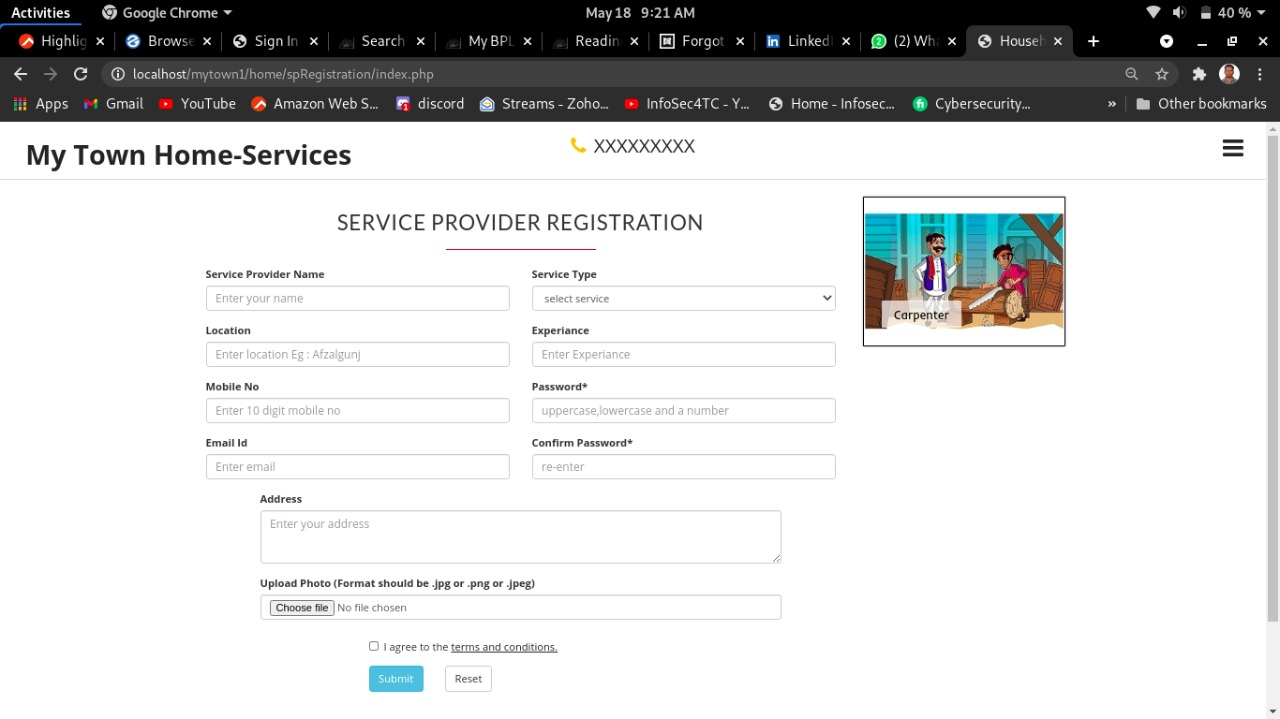
\includegraphics[width=1.0\linewidth,height=0.5\textheight]{sp.jpeg}
	\end{center}
	\caption{Registration of Service Provider in My Town Home Services}
\end{figure}

\textbf{ }
\textbf{ \hspace{15pt}}

\begin{figure}[h!]
	\begin{center}
		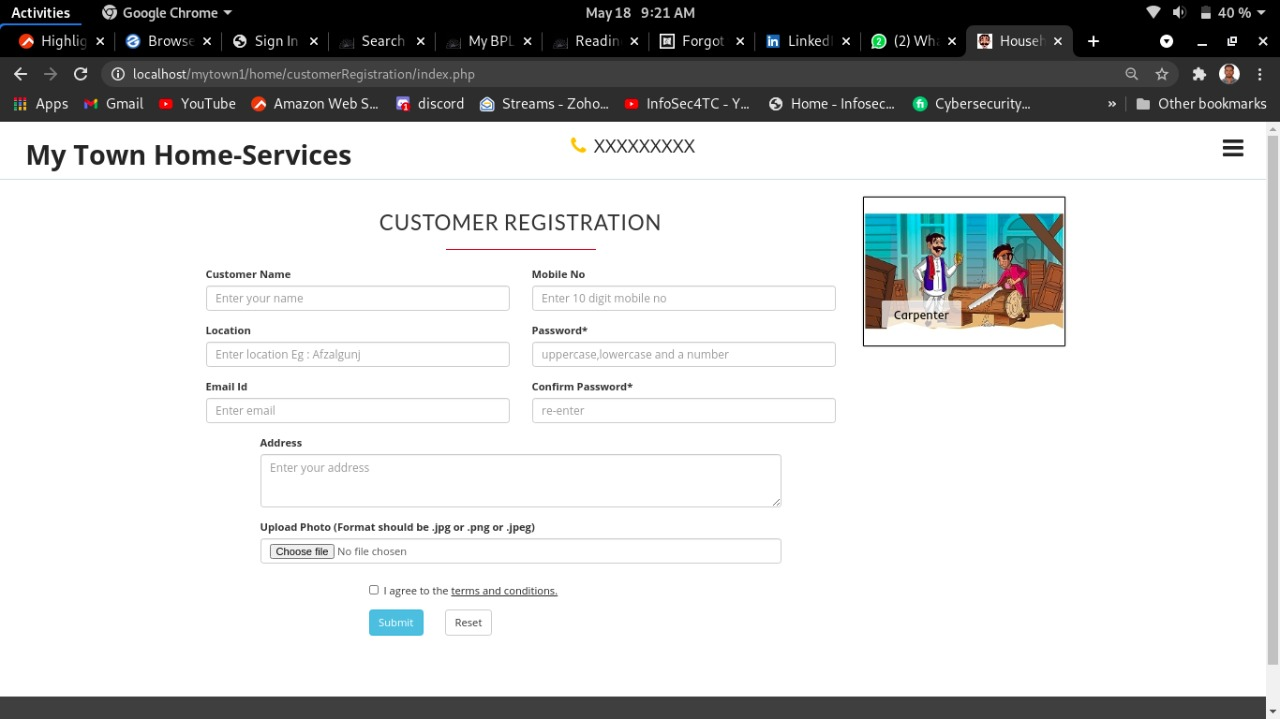
\includegraphics[width=\linewidth]{cust.jpeg}
	\end{center}
	\caption{Registration of Customer in My Town Home Services}
\end{figure}
\newpage
\raggedright
\subsection{ Testing for Searching and Display List of Service Providers }

\begin{figure}[h!]
	\begin{center}
		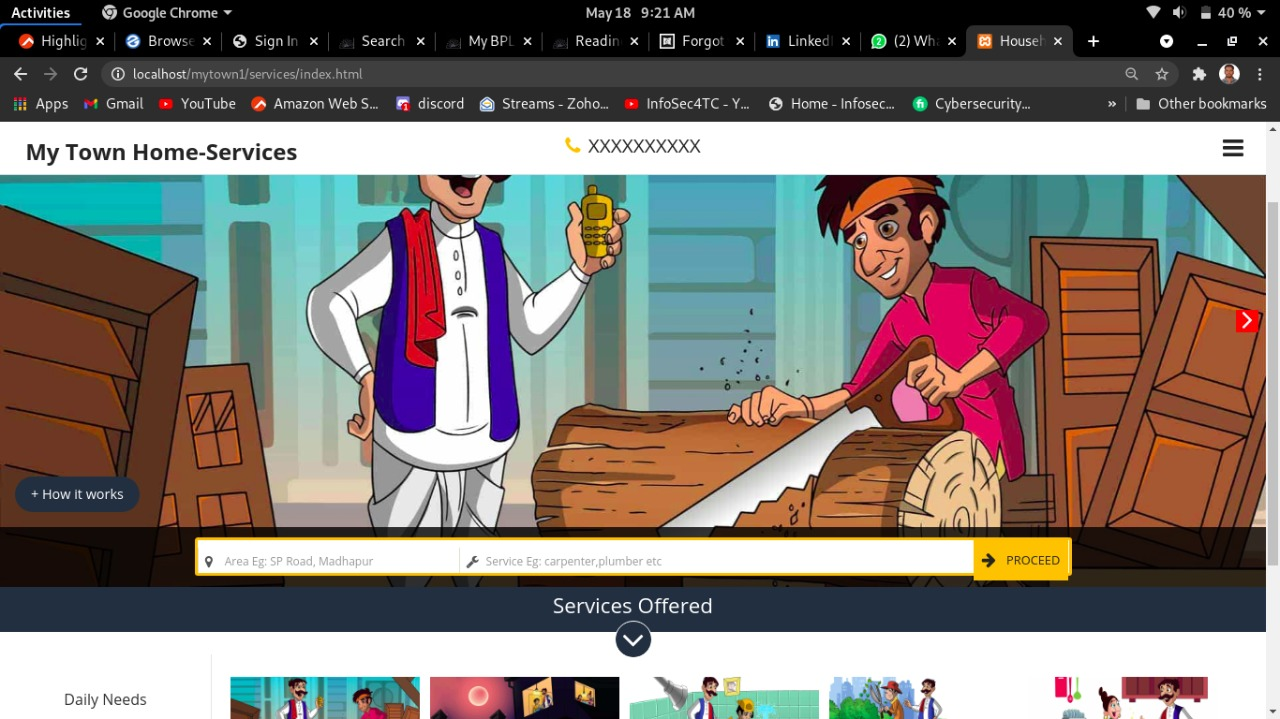
\includegraphics[width=\linewidth]{services.jpeg}
	\end{center}
	\caption{List of Service Providers in My Town Home Services}
\end{figure}
\begin{figure}[h!]
	\begin{center}
		 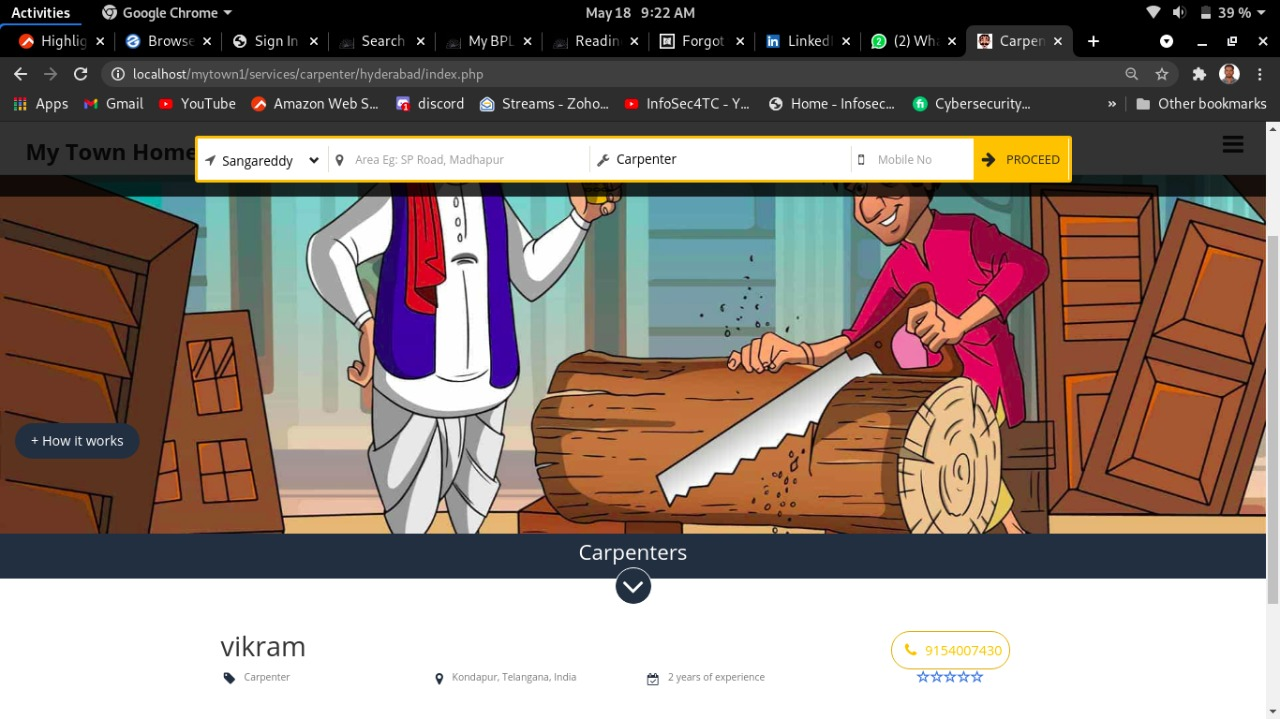
\includegraphics[width=\linewidth]{car.jpeg}
	\end{center}
	\caption{Carpenter Service Searching by Name in My Town Home Services}
\end{figure}
 
\vspace{0.75}
\raggedright
\subsection{ Testing for Reserve}\\ \\
\begin{figure}[h!]
	\begin{center}
		 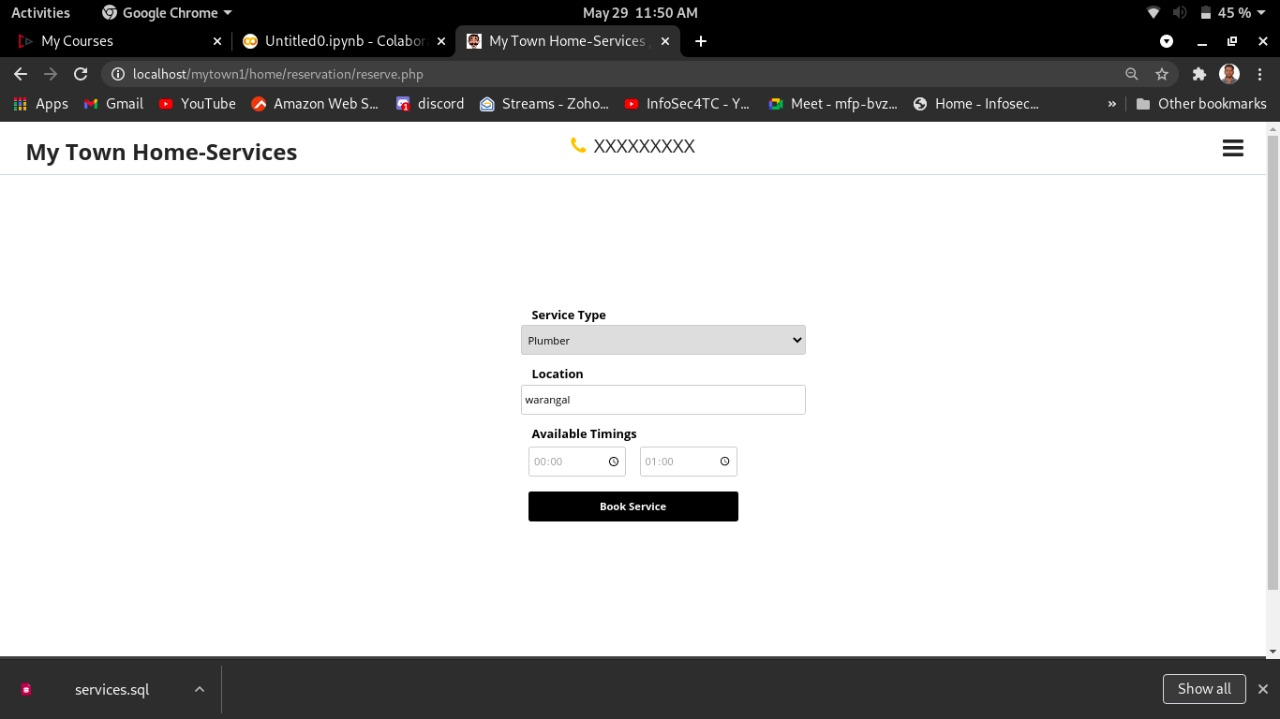
\includegraphics[width=\linewidth]{reserve.jpeg}
	\end{center}
	\caption{Reserving Service Provider in My Town Home Services}
\end{figure}
\newpage
{\raggedright
\chapter{ RESULTS }
}
Upon execution of the website code, below are the results we've obtained. The figures gives a clear picture of how well the web pages are organized namely the homepage, customer page, service provider page, search and display page and reserving page.
\newpage
\section{ Home Page}\\ [3.0cm]
\vspace{0.30cm}
\begin{figure}[h!]
	\begin{center}
		 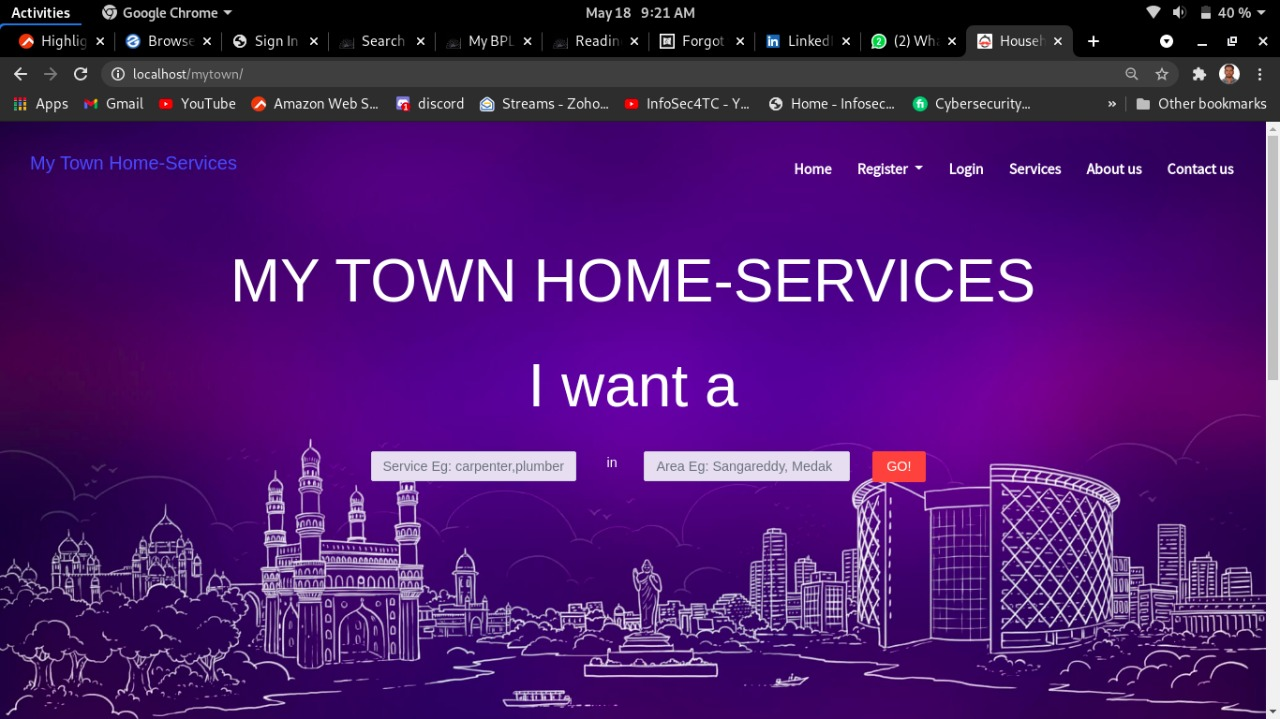
\includegraphics[width=1.0\linewidth,height=0.5\textheight]{home.jpeg}
	\end{center}
	\caption{Home Page in My Town Home Services}
\end{figure}
\newpage
{\raggedright
\section{ Service Provider Page}\\ \\[3.0cm]
\begin{figure}[h!]
	\begin{center}
		 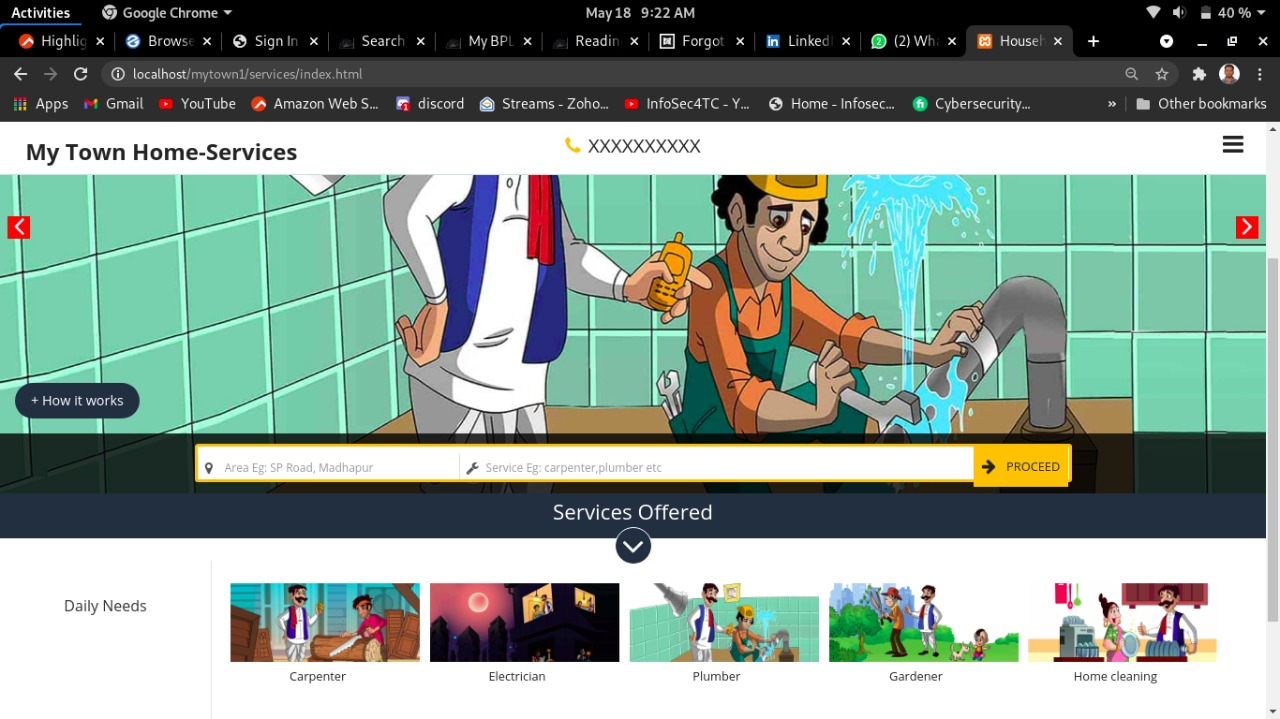
\includegraphics[width=1.0\linewidth,height=0.5\textheight]{plumber.jpeg}
	\end{center}
	\caption{Plumber Service in My Town Home Services}
\end{figure}
\raggedright

}

\newpage
\section{ Customer Page}\\[3.0cm]
\begin{figure}[h!]
	\begin{center}
		 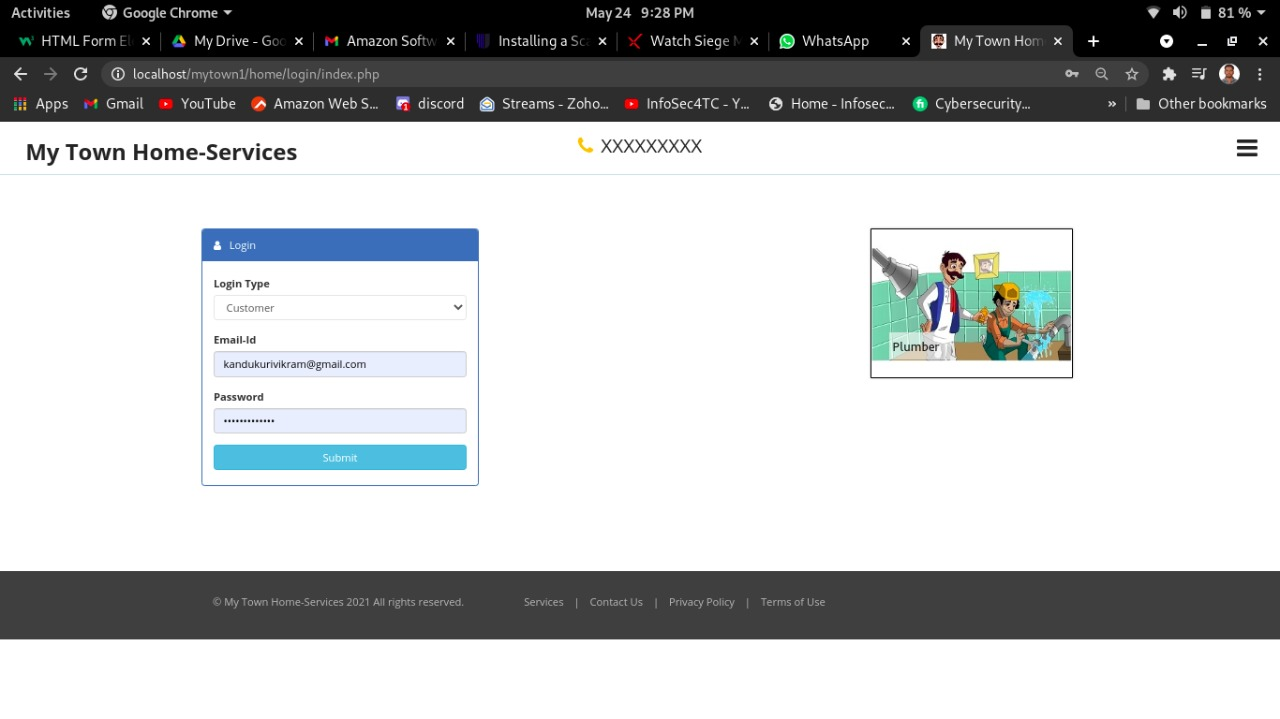
\includegraphics[width=1.0\linewidth,height=0.5\textheight]{custom.jpeg}
	\end{center}
	\caption{Customer Login Page in My Town Home Services}
\end{figure}

\newpage
\section{ Search and Display Page}\\[3.0cm]
\begin{figure}[h!]
	\begin{center}
		 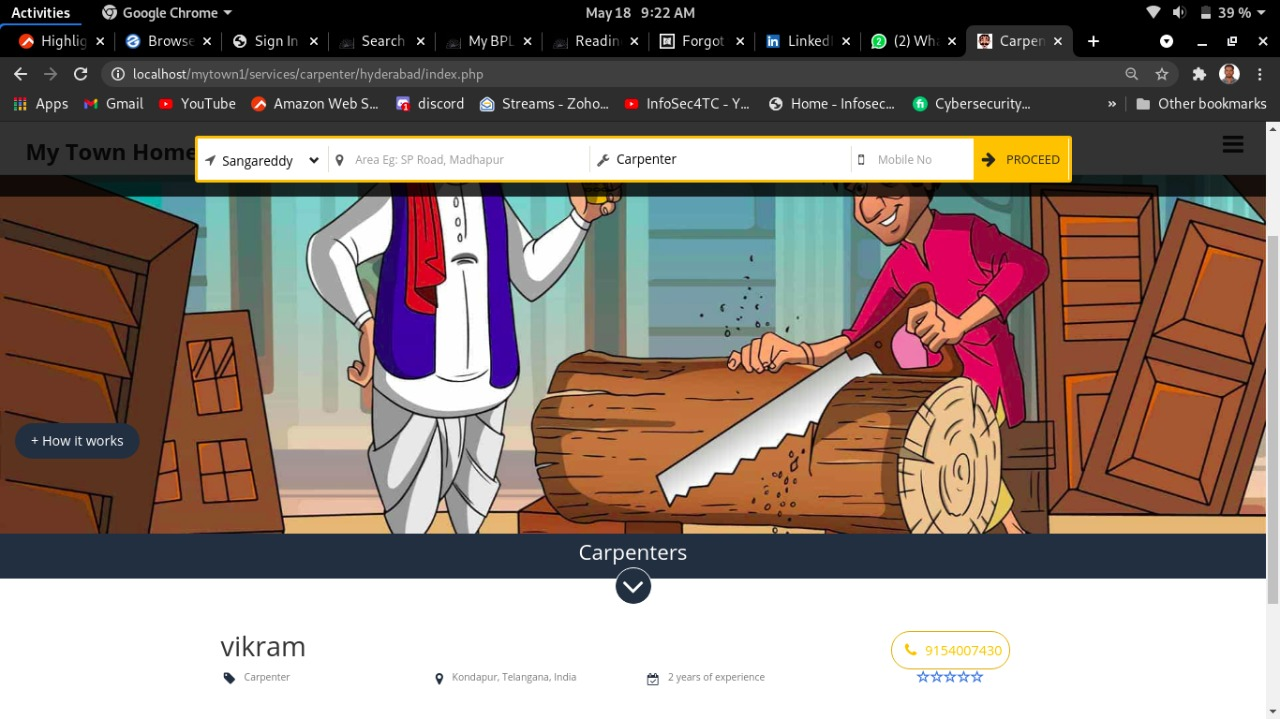
\includegraphics[width=1.0\linewidth,height=0.5\textheight]{car.jpeg}
	\end{center}
	\caption{Search and Display Page in My Town Home Services}
\end{figure}
\newpage

\textbf{ }\textbf{ }\textbf{ }\textbf{ }\textbf{ }\textbf{ }\textbf{ }\textbf{ }
\section{ Reserving Page}\\ \\[3.0cm]
\begin{figure}[h!]
	\begin{center}
		 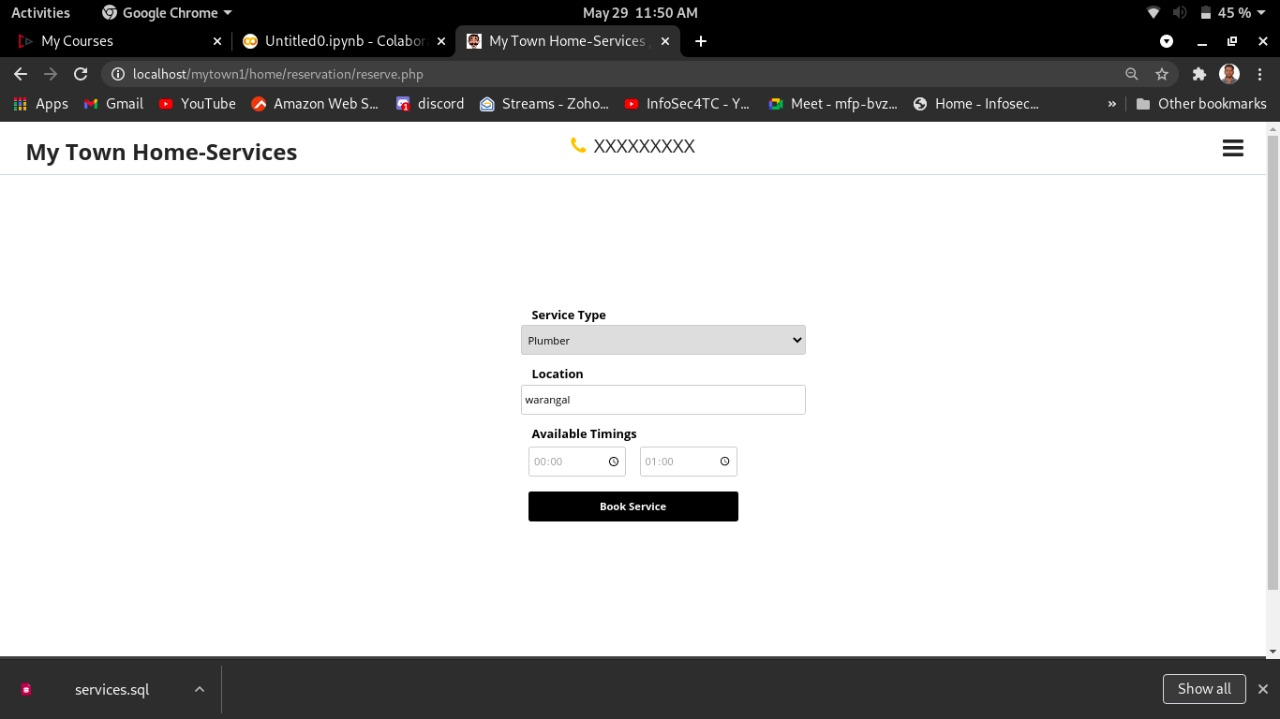
\includegraphics[width=\linewidth,height=0.5\textheight]{reserve.jpeg}
	\end{center}
	\caption{Reserving Service Provider Page in My Town Home Services}
\end{figure}
\textbf{ }
{\raggedright
\textbf{ }\textbf{ }
{\raggedright
\newpage
\addcontentsline{toc}{chapter}{FUTURE SCOPE}
\begin{center}
\LARGE \textbf{FUTURE SCOPE}\\[2.0cm]
\end{center}
For the enhancement of the website's effective performance , the data related to the service providers needs to be update, filtered and organized time to time updating it and monitoring it accordingly. The process is done automatically rendering the solutions with accuracy. The website can be further polished by including the features like upgradation of the user interface, details of the service providers and some course recommendations.\\  
Depending upon the functioning of the website at a wide level we can improve the security system and reassure the privacy of the customer.

\newpage

\addcontentsline{toc}{chapter}{CONCLUSION}
\begin{center}
\LARGE \textbf{CONCLUSION}\\[2.0cm]
\end{center}
We have implemented the provision of application to book service provider, thereby indicating that the proposed objective is well fit in implementing in the real word and be used by the people for the services. With more in-depth improvement and analysis of the search mechanism this website can  be  filtered to its best version of refinement. The website "My Town Home Services" shall diligently serve you with the best and desired quality and is reliable to use. The website provides independent professional and enterprise service providers as well. \\

"My Town Home Services" is the convenient path to figure out the best possible service available nearby saving the time of the customer and with the digitalization of the entire process.  \\
Service : ANYTIME and ANYWHERE
%\vspace{0.75cm}
\newpage
\addcontentsline{toc}{chapter}{REFERENCES}
\begin{center}
\LARGE \textbf{REFERENCES}\\[2.0cm]
\end{center}
\large
\begin{enumerate}[label={[\arabic*]}]

    \item \url{https://book-drive.com/learning-php-mysql-javascript/}
	\item \url{https://www.W3Schools.com/js/DEFAULT.asp}\\
    \item \url{https://www.quora.com/What-qualities-do-event-organizers-seek-in-conference-speakers}\\
    \item \url{https://www.click.in/hyderabad/ramukaka-household-services-carpenters-plumbers-electricians-c126-v19719747}\\
\end{enumerate}

\end{document}